\section{Algoritmo}\label{sec:algoritmo} 
Essa seção apresenta um algoritmo para gerar todos os cortes de Chvátal-Gomory de rank-1 e foi retirado
de \cite{Fischetti07}. A figura \ref{AlgoritmoRank1} apresenta esse algoritmo. Na linha 2 o modelo da seção
\ref{sec:modelagem} é relaxado, isto é, as variáveis $x$ agora pertencem ao intervalo $[0,1]$, e então é 
resolvido. Os laços das linhas 3 a 10 são executados até que uma solução inteira seja encontrada ou 
que o tempo máximo ocorra. A linha 3 verifica se a atual solução $x$ é inteira, caso positivo, nada mais 
precisa ser feito, caso negativo entra-se no loop. A linha 4 verifica se existe algum corte de 
Chvátal-Gomory de rank-1 que corta $x$, caso positivo a linha 5 adiciona o corte encontrado no 
modelo relaxado e a linha 6 resolve o modelo relaxado com esse novo corte. Caso nenhum corte seja
encontrado a linha 9 é executada e o algoritmo termina.
\begin{figure}
\centering
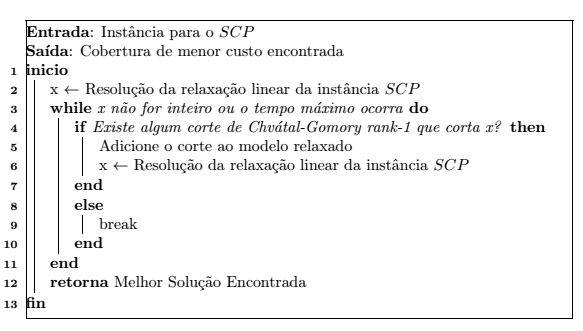
\includegraphics[width=4in]{AlgoritmoRank1.PNG}
\caption{Algoritmo para encontrar cortes de Chvátal-Gomory de rank-1 para o $SCP$}
\label{AlgoritmoRank1}
\end{figure}
Para verificar se existe algum corte de Chvátal-Gomory de rank-1 que corta uma solução fracionária
$x$ é utilizado um formulação de programação linear inteira mista baseada na formulação do problema de separação $np$-$dificil$ proposta em
\cite{Fischetti07}. A formulação
é composta pela função objetivo \eqref{eq:objetivo} e pelas restrições \eqref{eq:resticaoA}-\eqref{eq:inteira}.
\begin{align}
    & \text{min } \sum_{j \in N} \alpha_jx_j - \alpha_0 \label{eq:objetivo} \\
    & \text{Sujeito à:} \nonumber \\
    & 0 \le \alpha_j - u^TA_j  \le 1 -\delta \textrm{,} \forall j \in N \label{eq:resticaoA} \\ 
    & 0 \le \alpha_0 - u^Tb \le 1 -\delta \label{eq:b} \\
    & 0 \le u_i \le 1 -\delta \textrm{,} \forall i=1,...,m \label{eq:u} \\
    & \alpha_0 \le \sum_{j \in N} \alpha_j \textrm{,} \label{eq:mantem_binarias} \\
    & \alpha_0, \alpha_j \textrm{ inteiro, } \forall j \in N \label{eq:inteira}
\end{align}
Dada uma solução fracionária $x$ para o $SCP$, se a formulação anterior possui solução negativa,
então teremos $ \lceil u^TA_j \rceil x_j \le \lceil u^Tb \rceil$, então a restrição
$ \lceil u^TA_j \rceil x_j \ge \lceil u^Tb \rceil$ é um restrição válida para o $SCP$ que corta $x$. A restrição \eqref{eq:resticaoA},
juntamente com a restrição \eqref{eq:inteira} garantem que $\alpha_j$ é o menor inteiro, maior ou igual a $u^TA_j$,
ou seja $\alpha_j = \lceil u^TA_j \rceil$.
A restrição \eqref{eq:b},
juntamente com a restrição \eqref{eq:inteira} garantem que $\alpha_0$ é o menor inteiro, maior ou igual a $u^Tb$, ou seja
$\alpha_0 = \lceil u^Tb \rceil$. A restrição \eqref{eq:mantem_binarias} garante que os cortes gerados continuaram
a manter as variáveis $x$ com um valor máximo 1.